%
% ---------------------------------------------------------------
% Copyright (C) 2012-2018 Gang Li
% ---------------------------------------------------------------
%
% This work is the default powerdot-tuliplab style test file and may be
% distributed and/or modified under the conditions of the LaTeX Project Public
% License, either version 1.3 of this license or (at your option) any later
% version. The latest version of this license is in
% http://www.latex-project.org/lppl.txt and version 1.3 or later is part of all
% distributions of LaTeX version 2003/12/01 or later.
%
% This work has the LPPL maintenance status "maintained".
%
% This Current Maintainer of this work is Gang Li.
%
%

\documentclass[
 size=14pt,
 paper=smartboard,  %a4paper, smartboard, screen
 mode=present, 		%present, handout, print
 display=slides, 	% slidesnotes, notes, slides
 style=tuliplab,  	% TULIP Lab style
 pauseslide,
 fleqn,leqno]{powerdot}


\usepackage{cancel}
\usepackage{caption}
\usepackage{stackengine}
\usepackage{smartdiagram}
\usepackage{attrib}
\usepackage{amssymb}
\usepackage{amsmath} 
\usepackage{amsthm} 
\usepackage{mathtools}
\usepackage{rotating}
\usepackage{graphicx}

\usepackage{boxedminipage}
\usepackage{rotate}
\usepackage{calc}
\usepackage[absolute]{textpos}
\usepackage{psfrag,overpic}
\usepackage{fouriernc}
\usepackage{pstricks,pst-3d,pst-grad,pstricks-add,pst-text,pst-node,pst-tree}
\usepackage{moreverb,epsfig,subfigure}
\usepackage{color}
\usepackage{booktabs}
\usepackage{etex}
\usepackage{breqn}
\usepackage{multirow}
\usepackage{natbib}
\usepackage{bibentry}
\usepackage{gitinfo2}
\usepackage{siunitx}
\usepackage{nicefrac}
%\usepackage{geometry}
%\geometry{verbose,letterpaper}
\usepackage{media9}
\usepackage{animate}
%\usepackage{movie15}
\usepackage{auto-pst-pdf}

\usepackage{breakurl}
\usepackage{fontawesome}
\usepackage{xcolor}
\usepackage{multicol}



\usepackage{verbatim}
\usepackage[utf8]{inputenc}
\usepackage{dtk-logos}
\usepackage{tikz}
\usepackage{adigraph}
%\usepackage{tkz-graph}
\usepackage{hyperref}
%\usepackage{ulem}
\usepackage{pgfplots}
\usepackage{verbatim}
\usepackage{fontawesome}


\usepackage{todonotes}
% \usepackage{pst-rel-points}
\usepackage{animate}
\usepackage{fontawesome}

\usepackage{listings}
\lstset{frameround=fttt,
frame=trBL,
stringstyle=\ttfamily,
backgroundcolor=\color{yellow!20},
basicstyle=\footnotesize\ttfamily}
\lstnewenvironment{code}{
\lstset{frame=single,escapeinside=`',
backgroundcolor=\color{yellow!20},
basicstyle=\footnotesize\ttfamily}
}{}


\usepackage{hyperref}
\hypersetup{ % TODO: PDF meta Data
  pdftitle={Presentation Title},
  pdfauthor={Gang Li},
  pdfpagemode={FullScreen},
  pdfborder={0 0 0}
}


% \usepackage{auto-pst-pdf}
% package to show source code

\definecolor{LightGray}{rgb}{0.9,0.9,0.9}
\newlength{\pixel}\setlength\pixel{0.000714285714\slidewidth}
\setlength{\TPHorizModule}{\slidewidth}
\setlength{\TPVertModule}{\slideheight}
\newcommand\highlight[1]{\fbox{#1}}
\newcommand\icite[1]{{\footnotesize [#1]}}

\newcommand\twotonebox[2]{\fcolorbox{pdcolor2}{pdcolor2}
{#1\vphantom{#2}}\fcolorbox{pdcolor2}{white}{#2\vphantom{#1}}}
\newcommand\twotoneboxo[2]{\fcolorbox{pdcolor2}{pdcolor2}
{#1}\fcolorbox{pdcolor2}{white}{#2}}
\newcommand\vpspace[1]{\vphantom{\vspace{#1}}}
\newcommand\hpspace[1]{\hphantom{\hspace{#1}}}
\newcommand\COMMENT[1]{}

\newcommand\placepos[3]{\hbox to\z@{\kern#1S
        \raisebox{-#2}[\z@][\z@]{#3}\hss}\ignorespaces}

\renewcommand{\baselinestretch}{1.2}


\newcommand{\draftnote}[3]{
	\todo[author=#2,color=#1!30,size=\footnotesize]{\textsf{#3}}	}
% TODO: add yourself here:
%
\newcommand{\gangli}[1]{\draftnote{blue}{GLi:}{#1}}
\newcommand{\shaoni}[1]{\draftnote{green}{sn:}{#1}}
\newcommand{\gliMarker}
	{\todo[author=GLi,size=\tiny,inline,color=blue!40]
	{Gang Li has worked up to here.}}
\newcommand{\snMarker}
	{\todo[author=Sn,size=\tiny,inline,color=green!40]
	{Shaoni has worked up to here.}}

%%%%%%%%%%%%%%%%%%%%%%%%%%%%%%%%%%%%%%%%%%%%%%%%%%%%%%%%%%%%%%%%%%%%%%%%
% title
% TODO: Customize to your Own Title, Name, Address
%
\title{What's Cooking}
\author{
   Jincai Ma
\\
\\Xi'an Shiyou University}
\date{\today}


% Customize the setting of slides
\pdsetup{
% TODO: Customize the left footer, and right footer
rf=\href{http://www.tulip.org.au}{
Last Changed by: \textsc{\gitCommitterName}\ \gitVtagn-\gitAbbrevHash\ (\gitAuthorDate)
},
cf={What's Cooking},
}


\begin{document}

\maketitle

%\begin{slide}{Overview}
%\tableofcontents[content=sections]
%\end{slide}


%%==========================================================================================




%%==========================================================================================
%%
\begin{slide}{Introduction}
\begin{center}

{
\begin{itemize}
\item 
Use recipe ingredients to categorize the cuisine.\\
Given the name of the condiment, predict the cuisine to which the dish belongs.
\item In the dataset,  including the recipe ID, the dish, and the list of ingredients for each recipe (variable length).The data is stored in JSON format. \\
1.train.json- A training set that contains the recipe ID, dish type, and ingredient list
2.test.json- A test set containing a recipe ID and a list of ingredients
3.sample_submission.csv-Properly formatted sample submission document
\end{itemize}
}

\end{center}
\bigskip
\begin{center}

\end{center}
\bigskip

%%==========================================================================================

%%==========================================================================================

\end{slide}
%%
%%==========================================================================================



%%
\begin{slide}{Data Import And Introduction}
  \begin{center}

    {
      \begin{itemize}
        \item
        Import the JSON file with Pandas:
        We can get the data set of dish names, including 39774 training data and 9944 test samples.
        \item To see the distribution of our data set and the total variety of dishes, we printed out some of the data samples.
      \end{itemize}  
      
      \begin{figure}
        \centering
        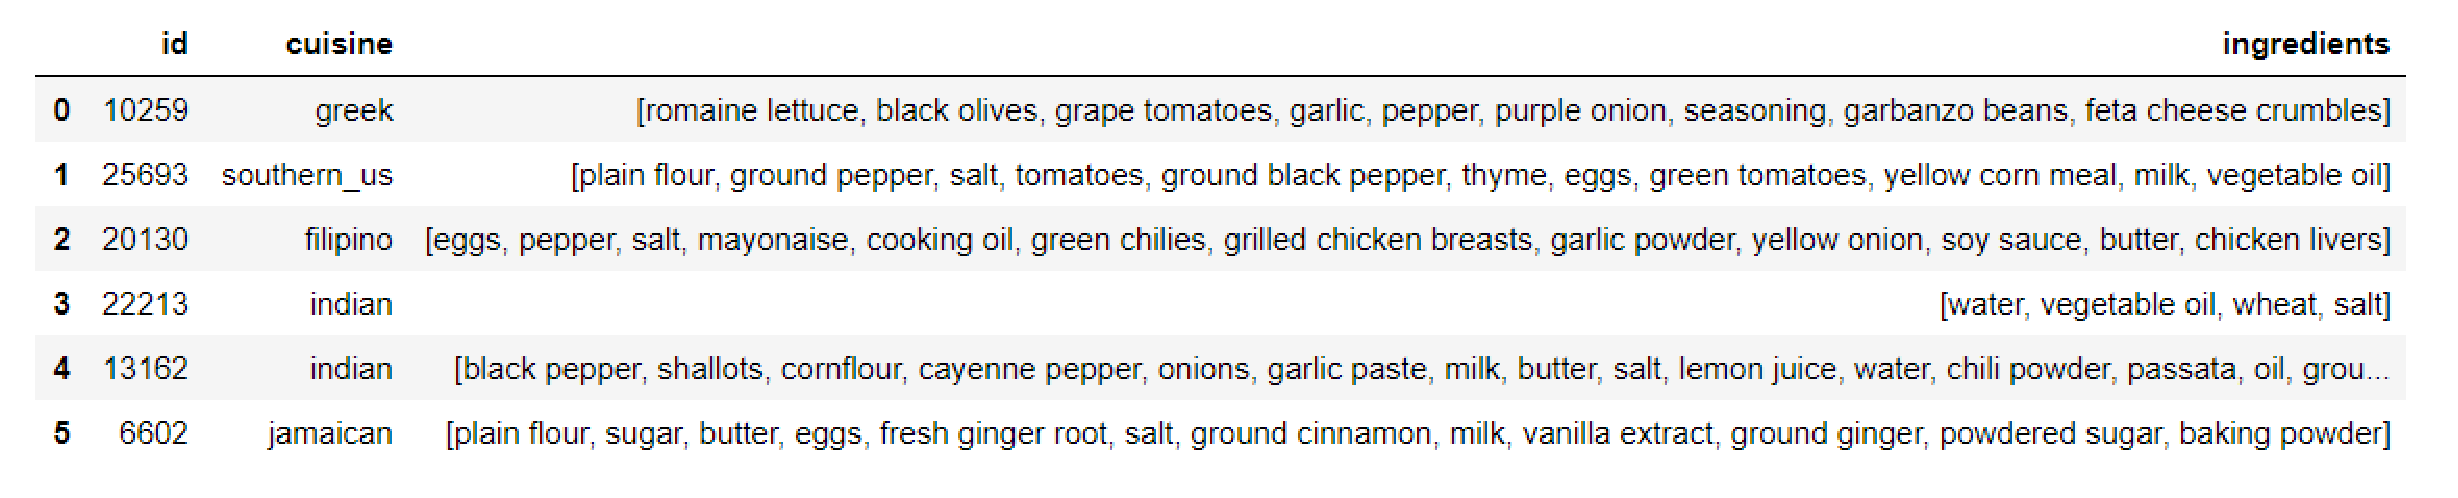
\includegraphics[width=0.9\textwidth]{pic01/a .eps}
      \end{figure}
      \begin{itemize}
        \item
        Total dish classification\\
        There are 20 dishes in total, which are:
        ['brazilian' 'british' 'cajun_creole' 'chinese' 'filipino' 'french'
         'greek' 'indian' 'irish' 'italian' 'jamaican' 'japanese' 'korean'
         'mexican' 'moroccan' 'russian' 'southern_us' 'spanish' 'thai'
         'vietnamese']
        
      \end{itemize}  
    
       
    }
    \end{center}
    \bigskip
    \begin{center}
    
    \end{center}
    \bigskip

%%==========================================================================================


%%==========================================================================================
\end{slide}
%%
%%==========================================================================================

%%==========================================================================================
%%
\begin{slide}{Analyze Data}
  \begin{center}

    {
      \begin{itemize}
      
        \item The data set is divided into Features and Target Variables.
        \item Features:'ingredients', we were given the names of the ingredients contained in each dish;
        Target variable:'cuisine', is the classification of cuisines that we want to predict.
        \item Extract the Feature of training data set into train\_integredients variable
              Extract the Target Variables into the train\_Targets variable
      \end{itemize} 
      
    
      \begin{figure}
        \centering
  
        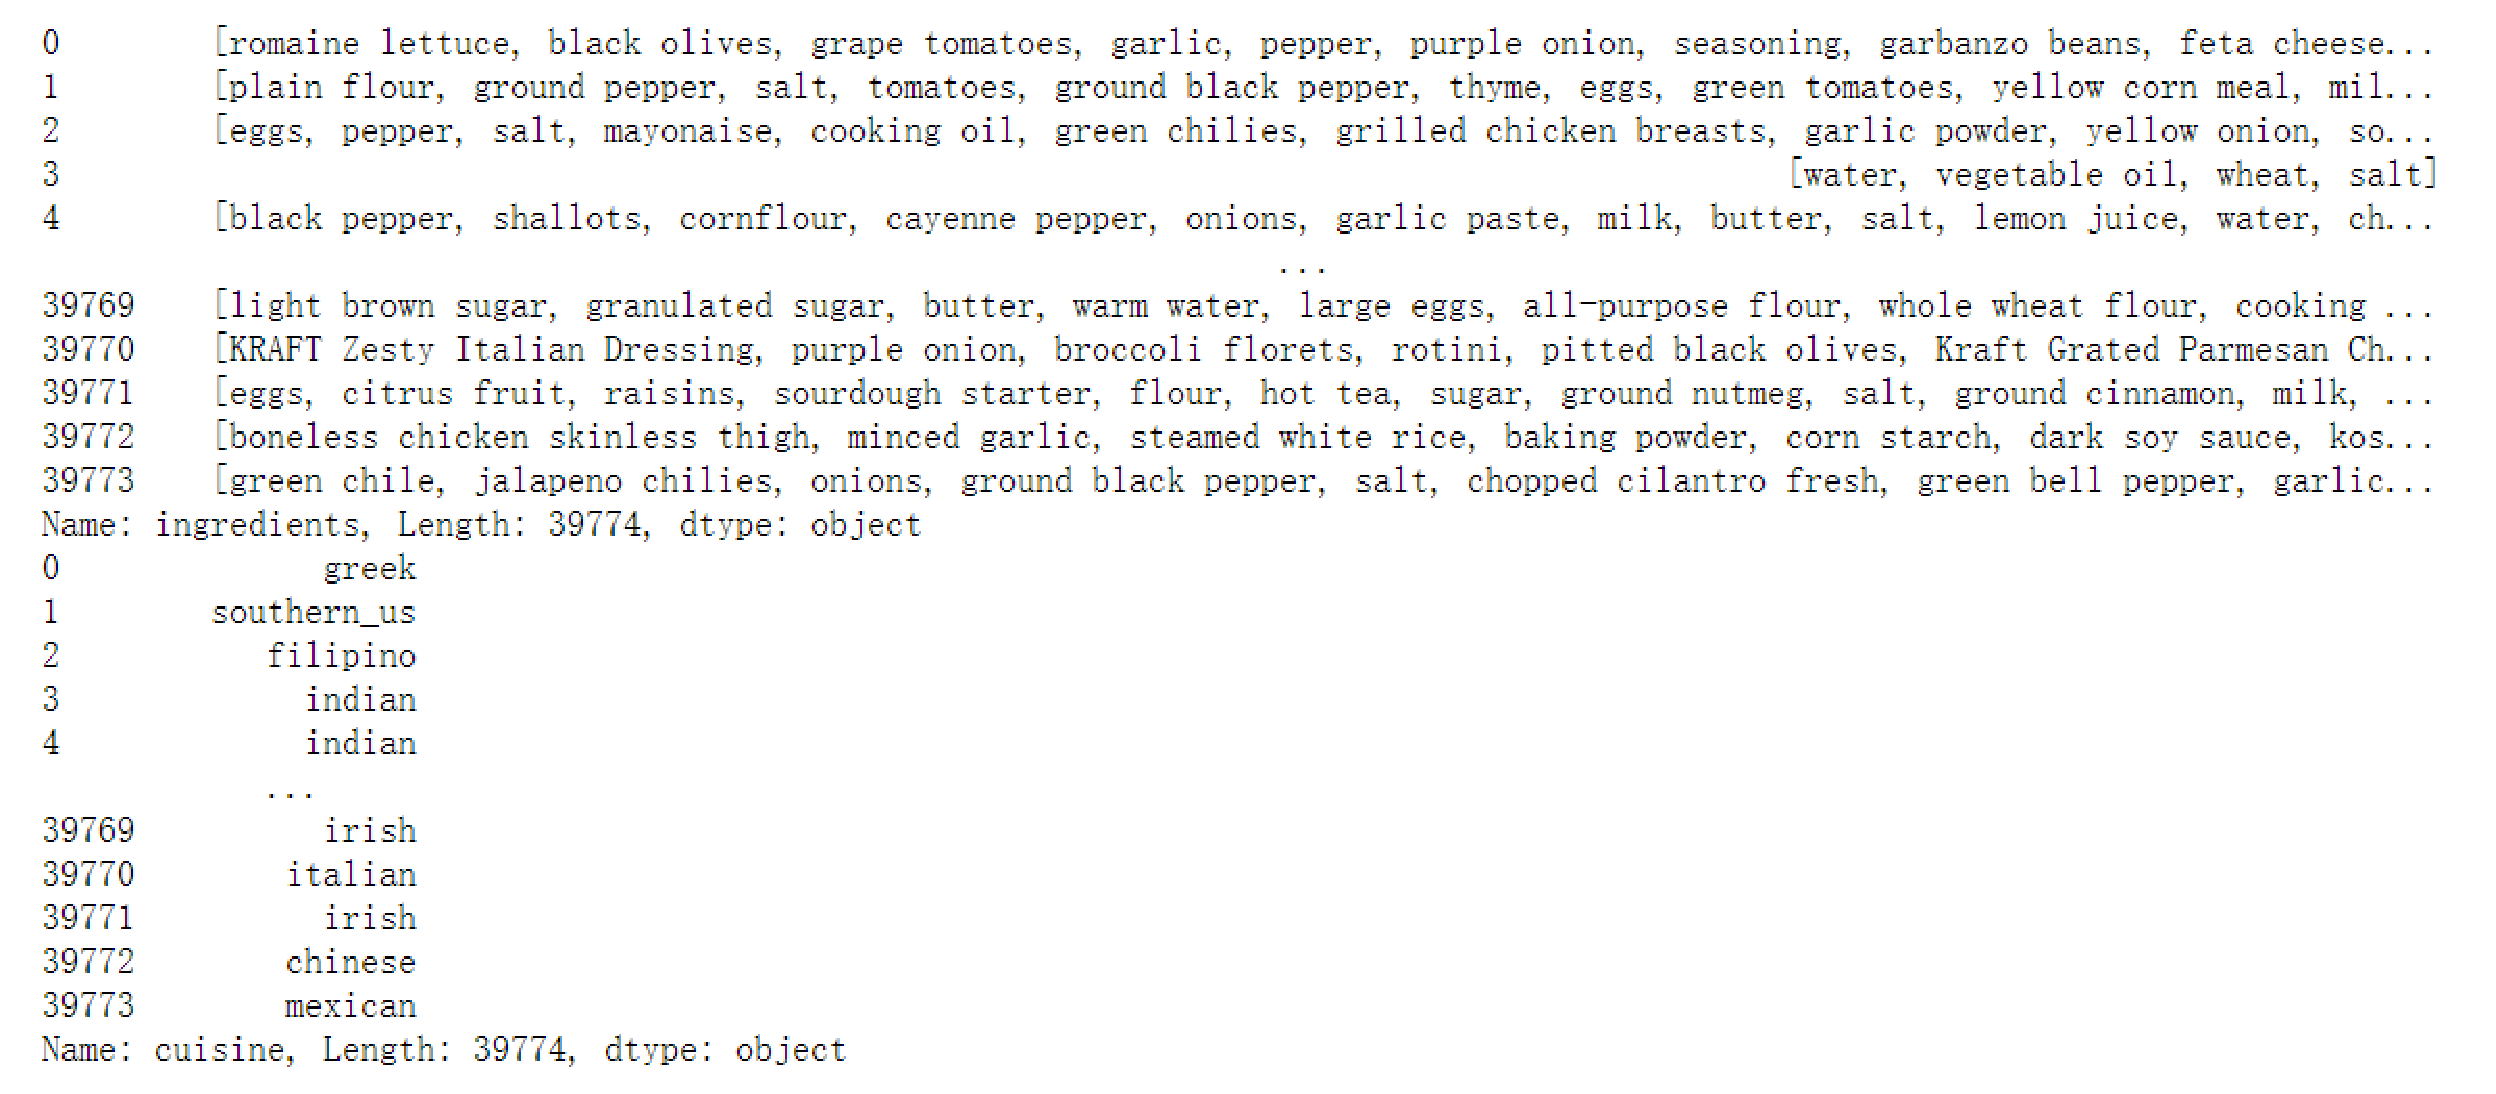
\includegraphics[width=0.6\textwidth]{pic01/b.eps} 
        
      \end{figure}   
        
       
    }
    \end{center}
  \bigskip
    \begin{center}
    
    \end{center}
  \bigskip



\end{slide}
%%
%%==========================================================================================
%%
\begin{slide}{Data  Visualization}
  \begin{center}

    {
      \begin{itemize}
      
        \item What are the top 10 most frequently used ingredients?
        \item What are the 10 most common ingredients in filipino,greek and Italian cuisine?
       
      \end{itemize} 
           
    
      \begin{figure}
        \centering
        \begin{minipage}[t]{0.45\textwidth}
        \centering
        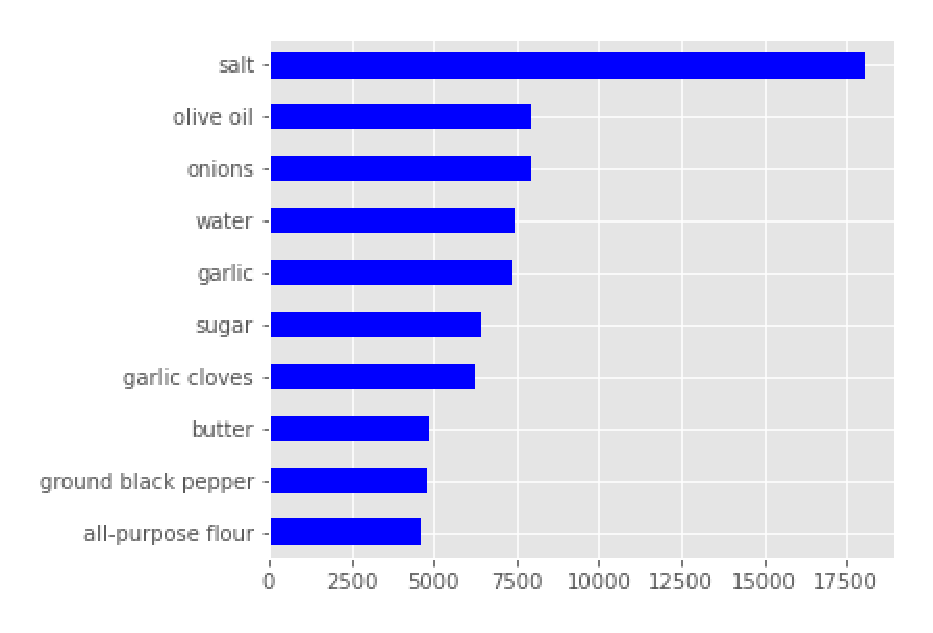
\includegraphics[width=0.6\textwidth]{pic01/cooking.eps} 
        \caption{sum}
        \end{minipage}
        \begin{minipage}[t]{0.45\textwidth}
        \centering
        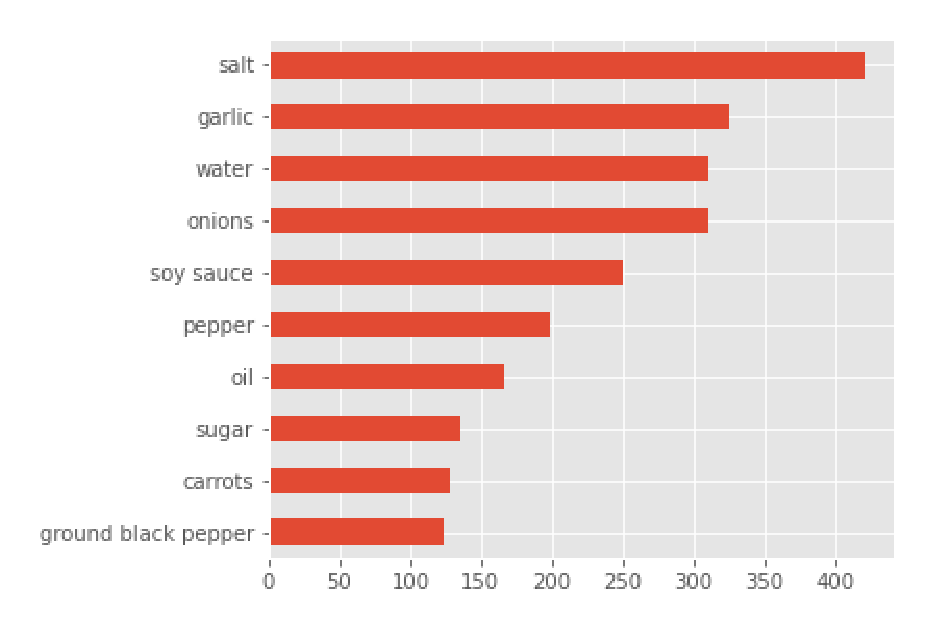
\includegraphics[width=0.6\textwidth]{pic01/filipino.eps}
        \caption{filipino}
        \end{minipage}
        \begin{minipage}[t]{0.45\textwidth}
        \centering
        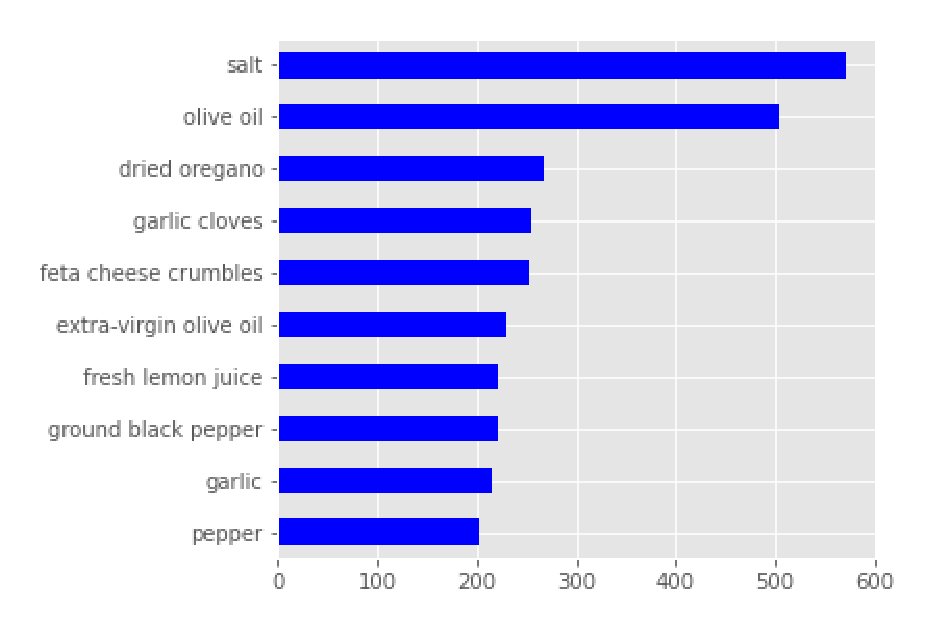
\includegraphics[width=0.57\textwidth]{pic01/greek.eps}
        \caption{greek}
        \end{minipage}
        \begin{minipage}[t]{0.45\textwidth}
        \centering
        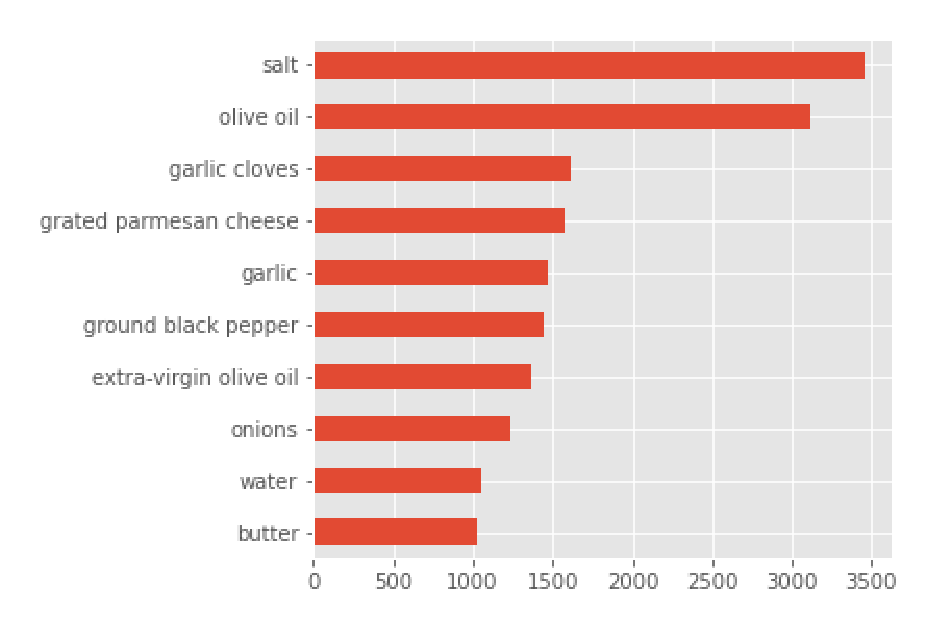
\includegraphics[width=0.57\textwidth]{pic01/italian.eps}
        \caption{italian}
        \end{minipage}
      \end{figure}   
        
    }
    \end{center}
  
    \bigskip
    \begin{center}
    
    \end{center}
  \bigskip

\end{slide}
%%
\section{Build Model}
%%==========================================================================================

\begin{slide}{Data Cleaning}
  \begin{center}
  
  {
  \begin{itemize}
  \item 
  Since dishes contain a large number of ingredients, and since the same ingredients can vary in numbers, tenses, and so on, we considered sifting through a potatos to remove any such differences
  \end{itemize}
  }
  \begin{figure}
    \centering
    \begin{minipage}[t]{1\textwidth}
    \centering
    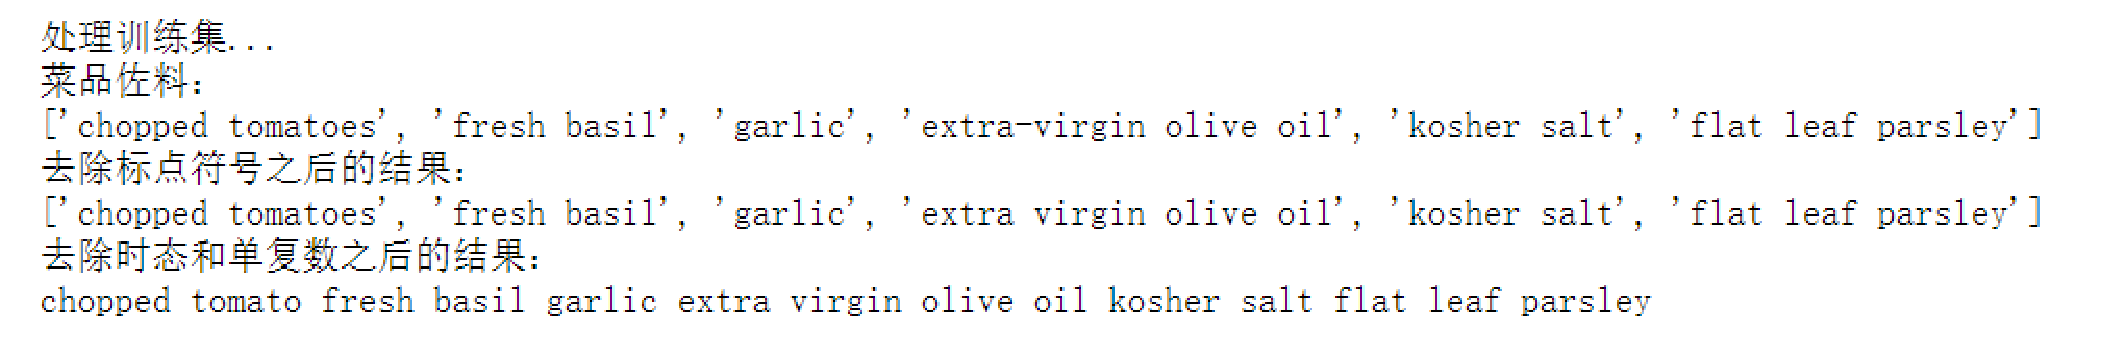
\includegraphics[width=0.7\textwidth]{pic01/clean1.eps} 
   
    \end{minipage}
    \begin{minipage}[t]{1\textwidth}
    \centering
    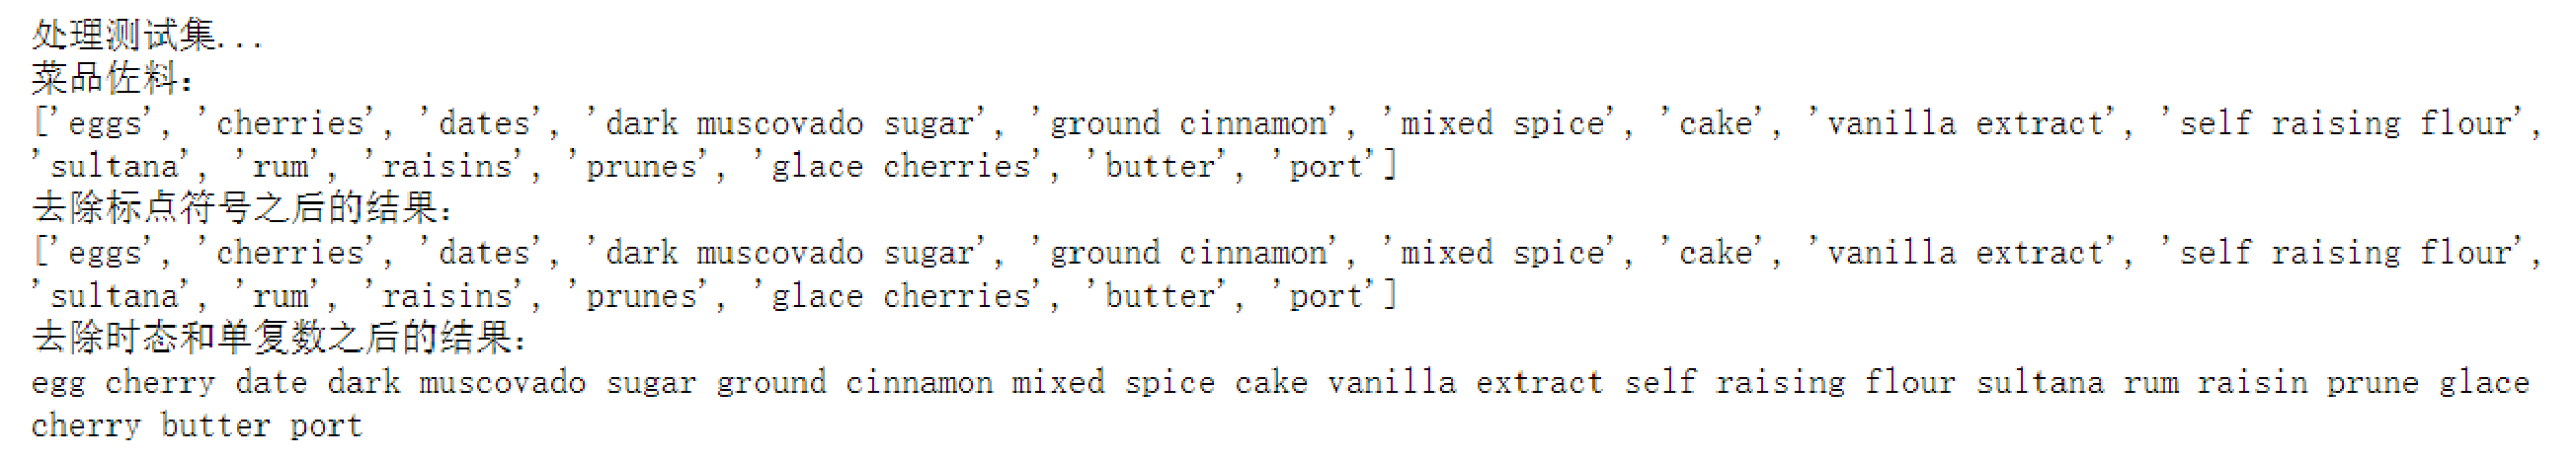
\includegraphics[width=0.7\textwidth]{pic01/clean2.eps}
   
    \end{minipage}
  \end{figure}   
    

  \end{center}
  \bigskip
  \begin{center}
  
  \end{center}
  \bigskip
  
  %%==========================================================================================
  
  %%==========================================================================================
  
  \end{slide}

%%
\begin{slide}{Feature extraction}
  \begin{center}
  
  {
    \begin{itemize}
     \item 
      We convert the ingredients of the dish into a numerical feature vector.Consider that most dishes include salt, water, sugar, butter, etc,We will consider weighting the seasonings according to the occurrence times of the seasonings, that is, the more the occurrence times of the condiments, the lower the discriminability of the condiments.The feature we adopt is TF-IDF.\\
     \item
      We can get the Top 10 characteristics:\lbrack'greek','southern\_us','filipino','indian','indian',\\
      'jamaican','spanish','italian','mexican','italian'\rbrack
     \item The top five data in train\_tfidf:\\
     \lbrack\lbrack0. 0. 0. ... 0. 0. 0.\rbrack\\
     \lbrack0. 0. 0. ... 0. 0. 0.\rbrack\\
     \lbrack0. 0. 0. ... 0. 0. 0.\rbrack\\
     \lbrack0. 0. 0. ... 0. 0. 0.\rbrack\\
     \lbrack0. 0. 0. ... 0. 0. 0.\rbrack\rbrack
    \end{itemize}
  }
  
  \end{center}
  \bigskip
  \begin{center}
  
  \end{center}
  \bigskip
  
  %%==========================================================================================
  
  %%==========================================================================================
  
  \end{slide}

\begin{slide}{Validation set partitioning}
  \begin{center}
  
    {
      \begin{itemize}
      \item 
       The training set is divided into a new training set and a validation set by calling train_test_split function, which is convenient for the subsequent accuracy observation of the model.
       \item
        1.Import train_test_split from sklear.model_selection\\
        2.Use train_tfidf and train_targets as input variables for train_test_split\\
        3.The test_size is set to 0.2, 20$\%$ of the validation set is divided, and 80$\%$ of the data is reserved for the new training set.\\
        4.Set the random_state random seed to ensure that the same partition results are obtained every time you run it.\\
     
      
      \end{itemize}
      }
  
  \end{center}
  \bigskip
  
\end{slide}
%%==========================================================================================
\begin{slide}{Training Model}
  \begin{center}
  
    {
      \begin{itemize}
      \item 
       Invoke the logistic regression model in sklearn.
      
      \item 
        1.Import the LogisticRegression from sklear.linear_model.\\
        2.GridSearchCV is imported from sklearn.model_selection, and the parameters are automatically searched. As long as the parameters are typed in, the best results and parameters can be given.\\
        3.Define the parameters variable: Create a dictionary for the C parameters, whose values are an array from 1 to 10;\\
        4.Define the classifier variable: Create a classification function using the imported LogisticRegression;\\
        5.Define Grid variables: Create a grid search object using the imported GridSearchCV;Pass the variables 'classifier', 'parameters' as arguments to the object constructor;\\
       
      \end{itemize}
      }
  
  \end{center}
  \bigskip
\end{slide}


\begin{slide}{The Results}
  \begin{center}
  
    {
      \begin{itemize}
       
        \item 
        After the model training, we calculated the prediction results of the model on the validation set X_VALID, and calculated the prediction accuracy of the model (compared with Y_VALID one by one).\\
        \item 
        The score on the validation set is: 0.7958516656191075.
      \end{itemize}
      }
  
  \end{center}
  \bigskip
\end{slide}
%%
\section{Model Predict}
\begin{slide}{Predictive test set}
  \begin{center}
  
  {
  \begin{itemize}
  \item 
  Test set test_tfidf is predicted by the model grid, and then the predicted results are viewed.\\
  The predicted number of test sets is 9944  
\end{itemize}
  }
  \begin{figure}
    \centering

    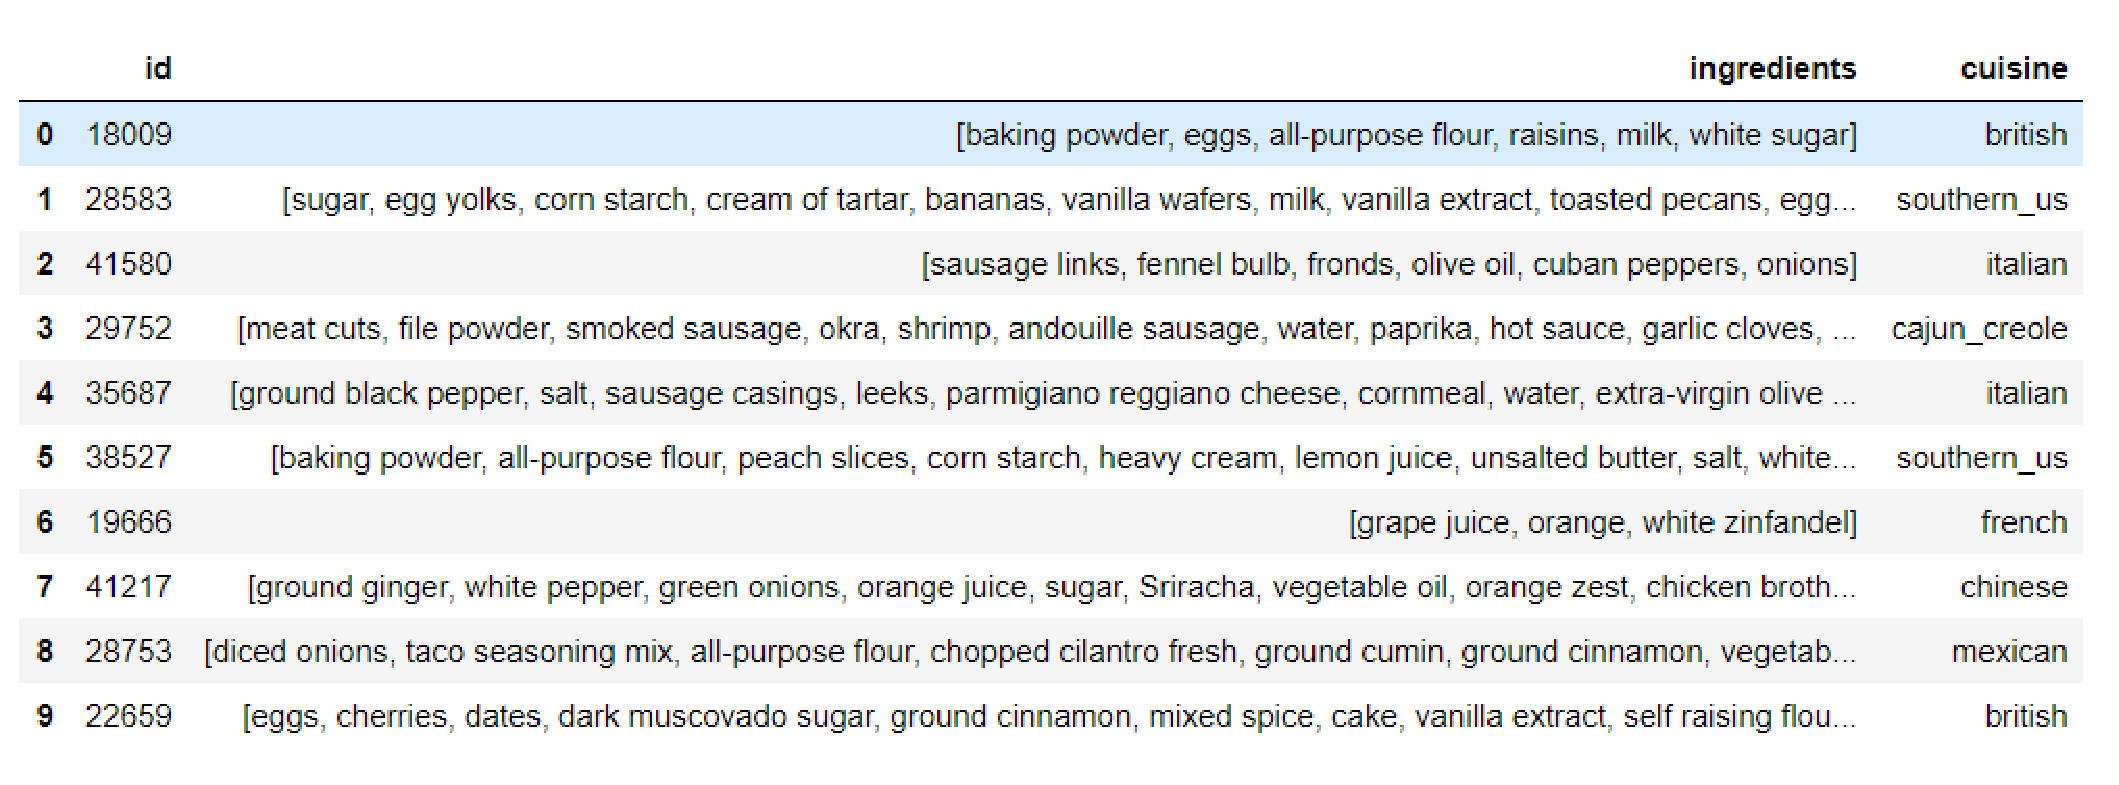
\includegraphics[width=0.6\textwidth]{pic01/result.eps} 
    
  \end{figure}   
     
    

  \end{center}
  \bigskip
  \begin{center}
  
  \end{center}
  \bigskip
\end{slide}
\end{document}

\endinput
